\newpage
\section{Implementierung (WIP)}\label{sec:implementation}

\subsection{App-Struktur (WIP)}
\textit{Eine kurze Beschreibung des Aufbaus der App}
\newline

\begin{figure}[h]
    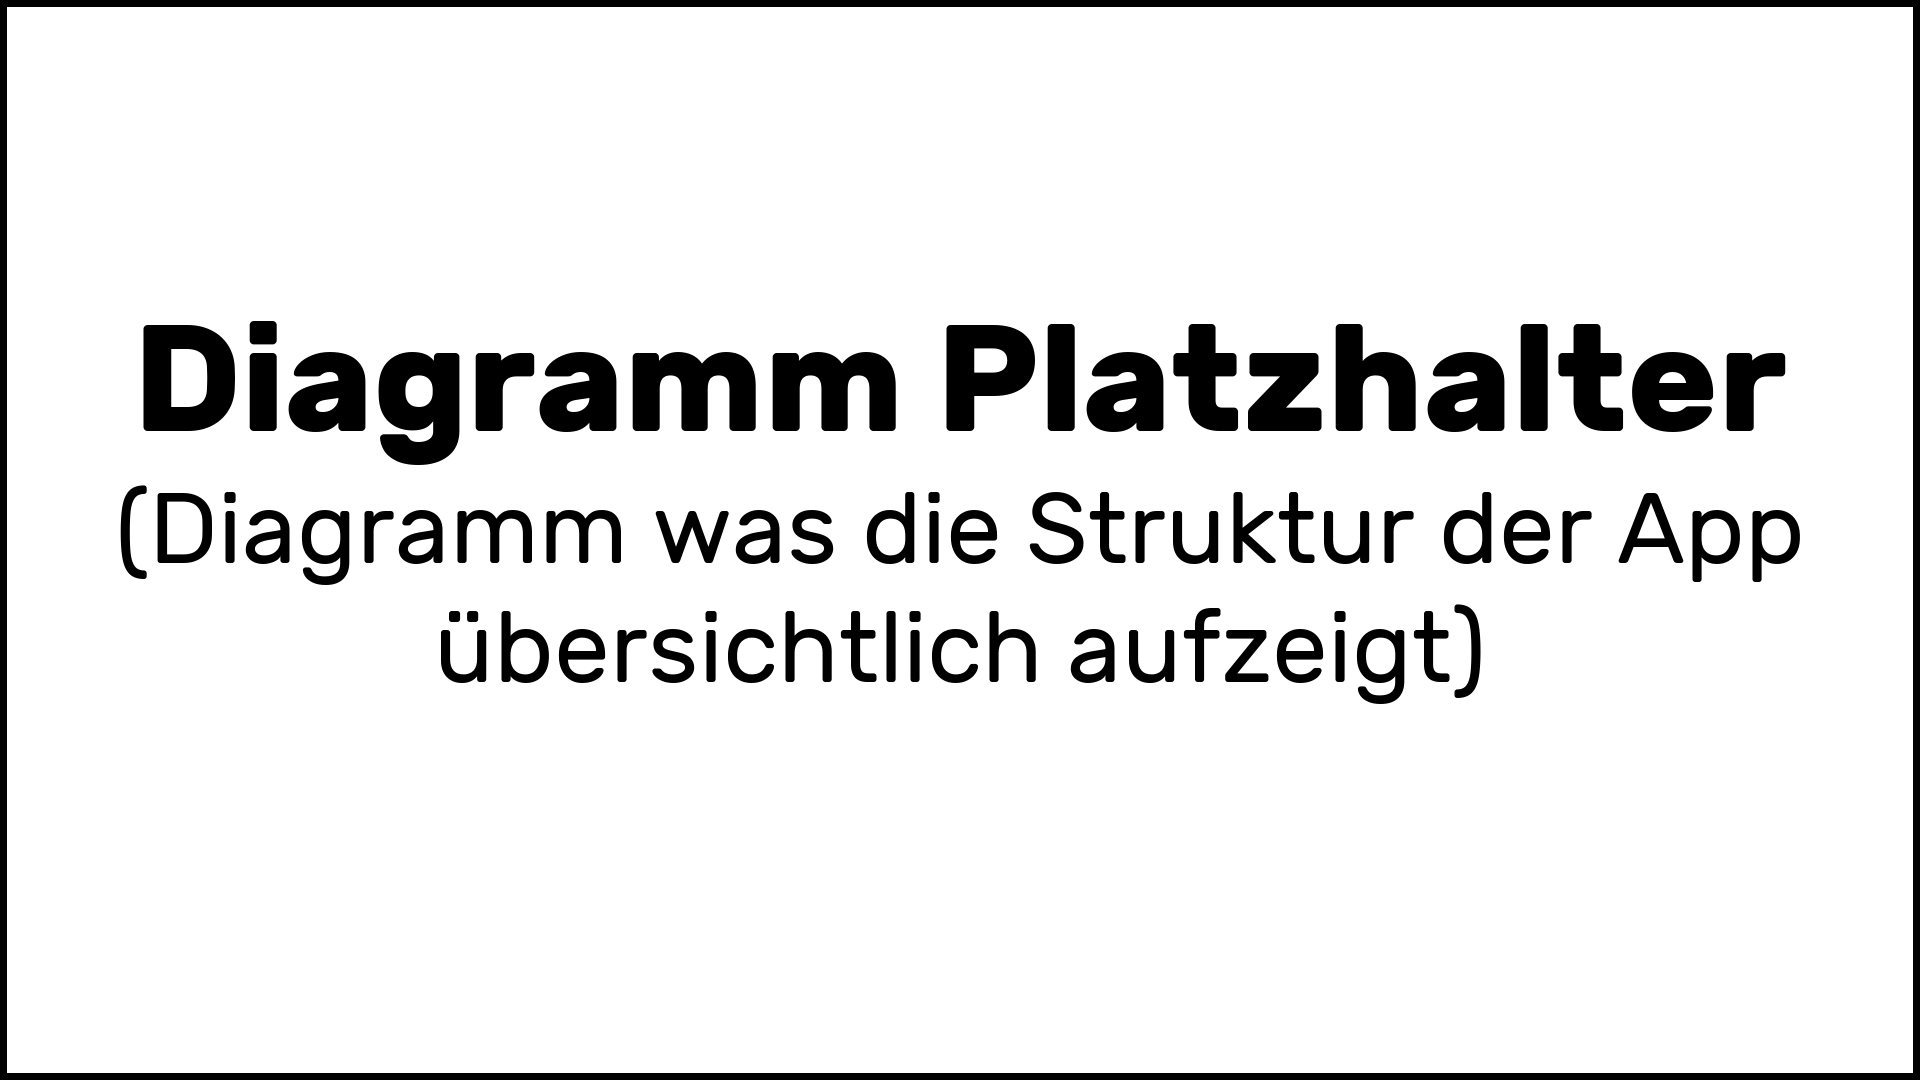
\includegraphics[width=\textwidth, center]{resources/diagram_structure.png}
    \caption[Diagramm: Aufbau der App]{Diagramm: Aufbau der App}
\end{figure}

\subsection{Grafische Bedienoberfläche (WIP)}
Unsere grafische Bedienoberfläche ist in drei Bereiche unterteilt: den Sprachverlauf, die Übersetzung und die Einstellungen. Das Farbschema lässt sich in den Einstellungen zwischen hell und dunkel umschalten. 

\begin{figure}[h]
    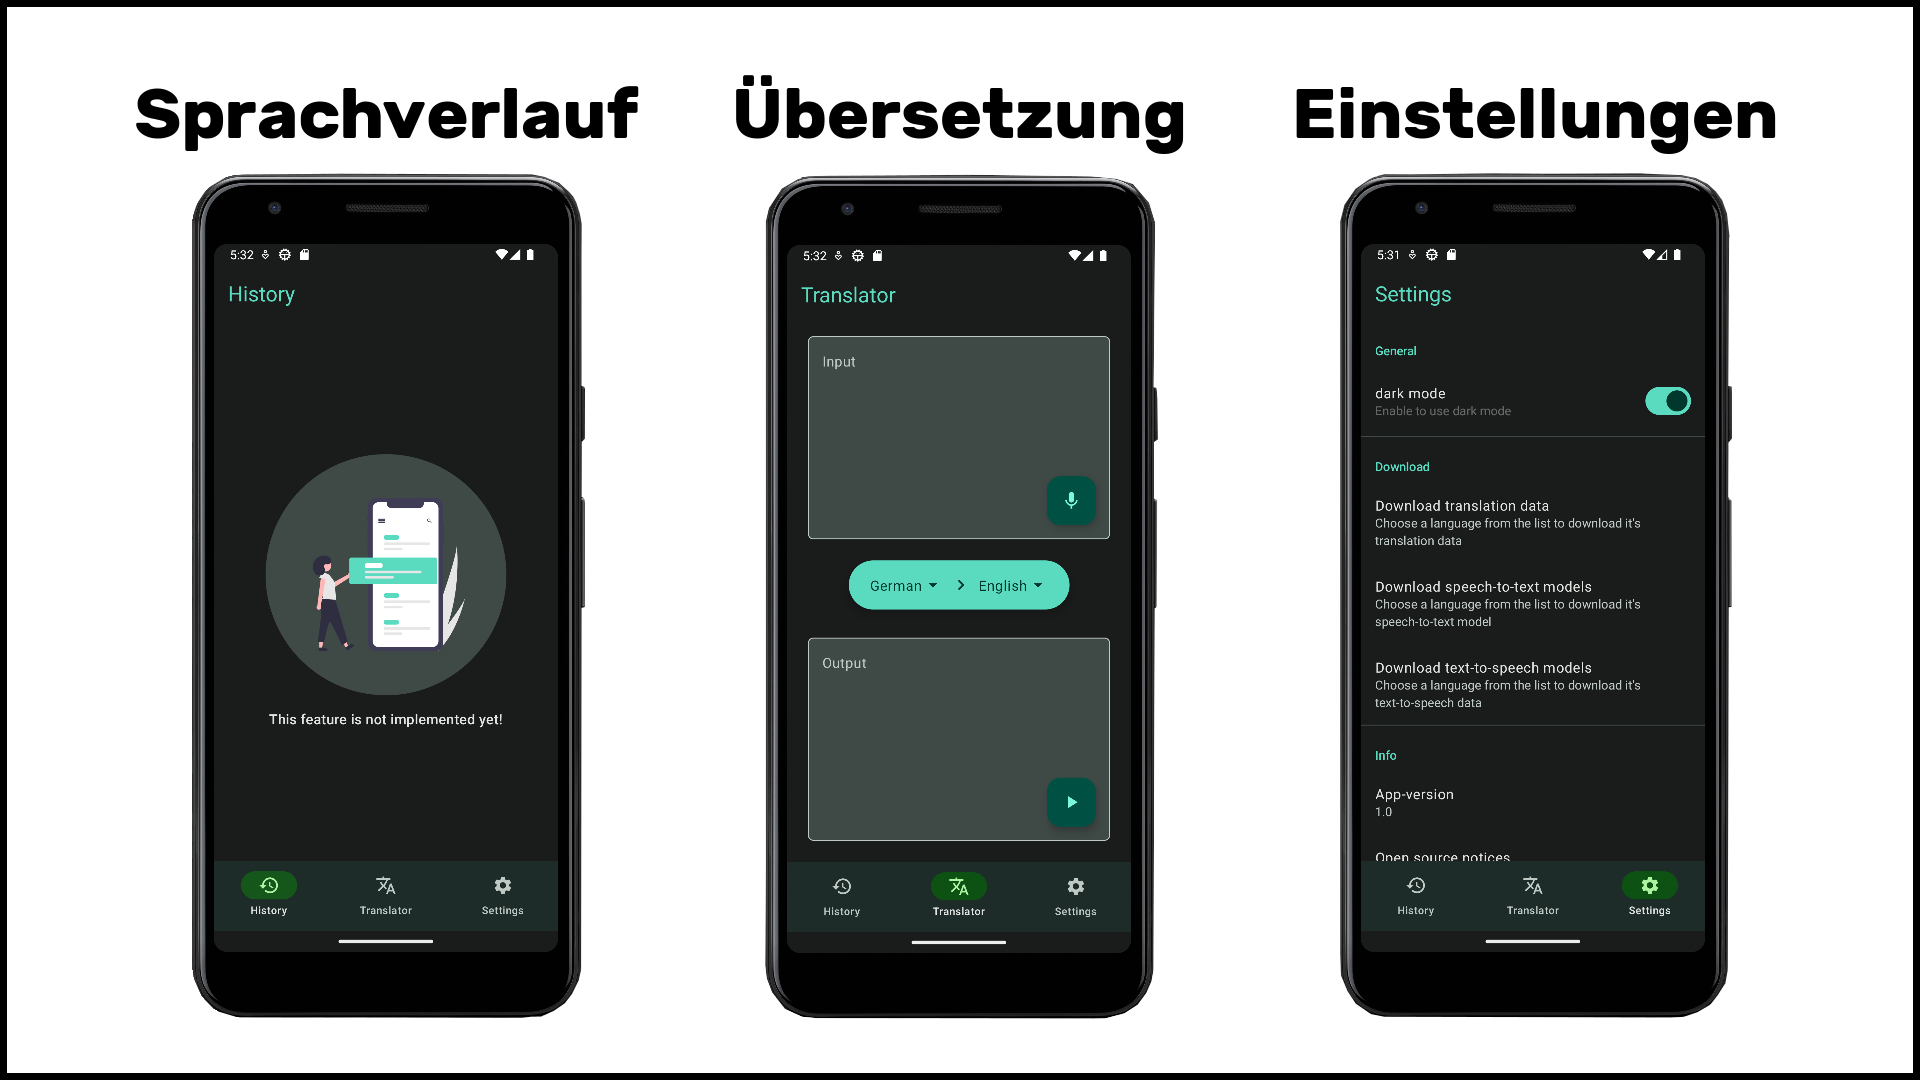
\includegraphics[width=\textwidth, center]{resources/diagram_graphics.png}
    \caption[Diagramm: Grafische Bedienoberfläche]{Diagramm: Grafische Bedienoberfläche}
\end{figure}


\subsubsection{Der Sprachverlauf (WIP)}
\textit{Eine genauere Beschreibung des Sprachverlaufs und seiner Funktionen.}

\subsubsection{Die Übersetzung (WIP)}
\textit{Eine genauere Beschreibung der Übersetzung und ihrer Funktionen.}

\subsubsection{Die Einstellungen (WIP)}
\textit{Eine genauere Beschreibung der Einstellungen und ihrer Funktionen.}

\subsection{Sprachein- und Ausgabe (WIP)}
Die Sprachein- und Ausgabe ist über den Android SpeechRecognizer sowie Android TextToSpeech umgesetzt. 
\newline
\newline
\textit{Genauer diskutieren, warum genau diese APIs für die Sprachein- und Ausgabe genutzt wurden.}

\subsection{Übersetzung (WIP)}
Die Übersetzung findet standardmäßig mit dem Google ML Kit Translator statt. Sollte eine Internetverbindung bestehen, wechselt die App automatisch auf den DeepL Übersetzer, um eine optimale Übersetzung zu gewährleisten.
\newline
\newline
\textit{Genauer diskutieren, warum genau diese APIs für die Übersetzung genutzt wurden.}